\documentclass{article}
\usepackage{iclr2018_conference, times}
\usepackage{hyperref}       % hyperlinks
\usepackage{url}            % simple URL typesetting
\usepackage{booktabs}       % professional-quality tables
\usepackage{amsfonts}       % blackboard math symbols
\usepackage{nicefrac}       % compact symbols for 1/2, etc.
\usepackage{microtype}      % microtypography
\usepackage{amsmath}
\usepackage{hyperref}
\usepackage{graphicx}
\usepackage{algorithm}
\usepackage{algpseudocode}
\usepackage{algorithm}
\usepackage{subcaption}
\usepackage{algpseudocode}
\usepackage{bm}
% rename algorithmic labels
\renewcommand{\algorithmicensure}{\textbf{return}}
\renewcommand{\algorithmicfunction}{\textbf{def}}

\definecolor{mydarkblue}{rgb}{0,0.08,0.45}
\hypersetup{colorlinks=true,
    linkcolor=mydarkblue,
    citecolor=mydarkblue,
    filecolor=mydarkblue,
    urlcolor=mydarkblue}

\newcommand{\vtheta}{\mathbf{\theta}}
\newcommand{\relaxed}{r}
\newcommand{\controlf}{\hat g}  % Control variate for functions
\newcommand{\controlg}{\hat g}  % Control variate for gradients
\newcommand{\discreteDist}{p(b|\theta)}
\newcommand{\loss}{f(b)}
\newcommand{\lossGrad}{\loss{} \frac{\partial}{\partial \theta }\log \discreteDist{}}
\newcommand{\mcGrad}{\hat{g}}
\newcommand{\expectedLoss}{\mathbb{E}_{\discreteDist{}} \! \left[ \, \loss{} \right]}
\newcommand{\expectedLossLogTrick}{\mathbb{E}_{\discreteDist{}} \! \left[ \, \lossGrad{} \right]}
\newcommand{\var}{\mathbb{V}}
\newcommand{\vu}{\mathbf{u}}
\newcommand{\E}{\mathbb{E}}
\newcommand{\LL}[1]{\frac{\partial \log \pi(a_{#1}| s_{#1}, \theta)}{\partial \theta}}
\newcommand{\PT}{\frac{\partial}{\partial \theta}}
\newcommand{\PP}[1]{\frac{\partial}{\partial #1}}
\newcommand{\PPH}{\frac{\partial}{\partial \phi}}
\newcommand{\LP}[1]{\PT \log p(#1)}
\newcommand{\LZ}[1]{\frac{\log \pi(z_{#1}| s_{#1}, \theta)}{\partial \theta}}

\newcommand{\YW}[1]{{\color{red} \bf [[YW: #1]]}}
\newcommand{\LAX}{{\textnormal{LAX}}}
\newcommand{\RL}{{\textnormal{RL}}}
\newcommand{\RELAX}{{\textnormal{RELAX}}}
\newcommand{\BAR}{{\textnormal{BAR}}}
\newcommand{\REBAR}{{\textnormal{REBAR}}}


\title{Backpropagation through the Void:\\
Optimizing control variates for black-box gradient estimation}
% Optimizing gradient control variates\\ for black-box expectations}

\author{
  Will S. Grathwohl\thanks{Use footnote for providing further
    information about author (webpage, alternative
    address)---\emph{not} for acknowledging funding agencies.} \\
  University of Toronto\\
  Vector Institute\\
  Toronto, ON \\
  \texttt{wgrathwohl@cs.toronto.edu} \\
}

\begin{document}
\maketitle
\begin{abstract}
Gradient-based optimization is the foundation of deep learning and reinforcement learning.
Even when the mechanism being optimized is unknown or not differentiable, optimization using high-variance or biased gradient estimates is still often the best strategy.
We introduce a general framework for learning low-variance, unbiased gradient estimators for black-box functions of random variables.
These estimators can be jointly trained with model parameters or policies, and are applicable in both discrete and continuous settings.
We give unbiased, adaptive analogs of state-of-the-art reinforcement learning methods such as advantage actor-critic.
We also demonstrate this framework for training discrete latent-variable models.
\end{abstract}


\section{Introduction}
Gradient-based optimization has been key to most recent advances in machine learning and reinforcement learning.
The back-propagation algorithm \citep{rumelhart1986learning}, also known as reverse-mode automatic differentiation~\citep{speelpenning1980compiling, rall1981automatic} computes exact gradients of deterministic, differentiable objective functions.
The reparameterization trick \citep{williams1992simple, kingma2013autoencoding, rezende2014stochastic} allows backpropagation to give unbiased, low-variance estimates of gradients of expectations of continuous random variables.
This has allowed effective stochastic optimization of large probabilistic latent-variable models.

%Unfortunately, backpropagation cannot be easily applied to problems involving discrete random variables, or when the function being optimized is a black box~\citep{schulman2015gradient}.
Unfortunately, there are many objective functions relevant to the machine learning community for which backpropagation cannot be applied. In reinforcement learning, for example, the function being optimized is unknown to the agent and is treated as a black box~\citep{schulman2015gradient}. Similarly, when fitting probabilistic models with discrete latent variables, discrete sampling operations create discontinuities giving the objective function zero gradient with respect to its parameters.
%This is the case in most reinforcement learning settings, or when fitting probabilistic models with discrete latent variables.
Much recent work has been devoted to constructing gradient estimators for these situations.
In reinforcement learning, advantage actor-critic methods~\citep{sutton2000policy} give unbiased gradient estimates with reduced variance obtained by jointly optimizing the policy parameters with an estimate of the value function.
In discrete latent-variable models, low-variance but biased gradient estimates can be given by continuous relaxations of discrete variables~\citep{maddison2016concrete, jang2016categorical}.

A recent advance by \citet{tucker2017rebar} used a continuous relaxation to construct a control variate for functions of discrete random variables. Low-variance estimates of the expectation of the control variate can be computed using the reparameterization trick to produce an unbiased estimator with lower variance than previous methods.
Furthermore, \citet{tucker2017rebar} showed how to tune the free parameters of these relaxations to minimize their variance during training.

%\paragraph{Contributions}
In this work we generalize the method of \citet{tucker2017rebar} to learn a free-form control variate parameterized by a neural network, giving a lower-variance, unbiased gradient estimator which can be applied to a wider variety of problems with greater flexibility.
Most notably, our method is applicable even when no continuous relaxation is available, as in reinforcement learning or black box function optimization.
Furthermore, we derive improved variants of popular reinforcement learning methods with unbiased, action-dependent gradient estimates and lower variance.%, and more stable training dynamics.

%\paragraph{Contributions}
%\begin{itemize}
%\item we keep conditional reparam from rebar while exploring and expanding on gradient signal for minimizing variance of estimator
%\item we generalize the concrete and muprop relaxations for a learnable family of functions that can be optimized via gradient decent to minimize the variance of the estimator
%\item We show that concrete relax is not optimal, and that control variate based on the discrete objective at continuous input is is not the optimal control variate.
%\item we combine these insights into a new family of estimators that generalizes rebar
%\end{itemize}

\begin{figure}[h]
\begin{center}
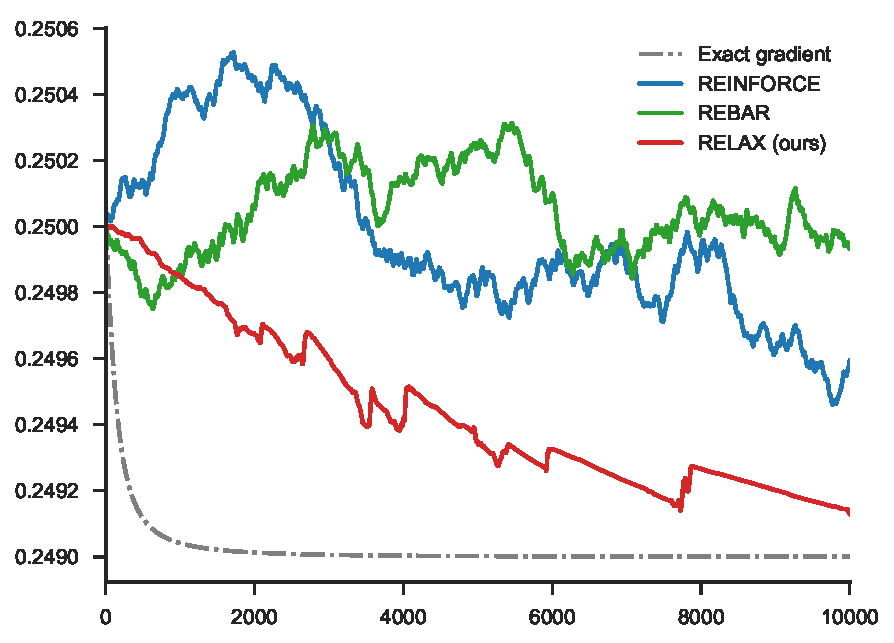
\includegraphics[width=.3\textwidth]{figures/toy_losses_10000_0_499}
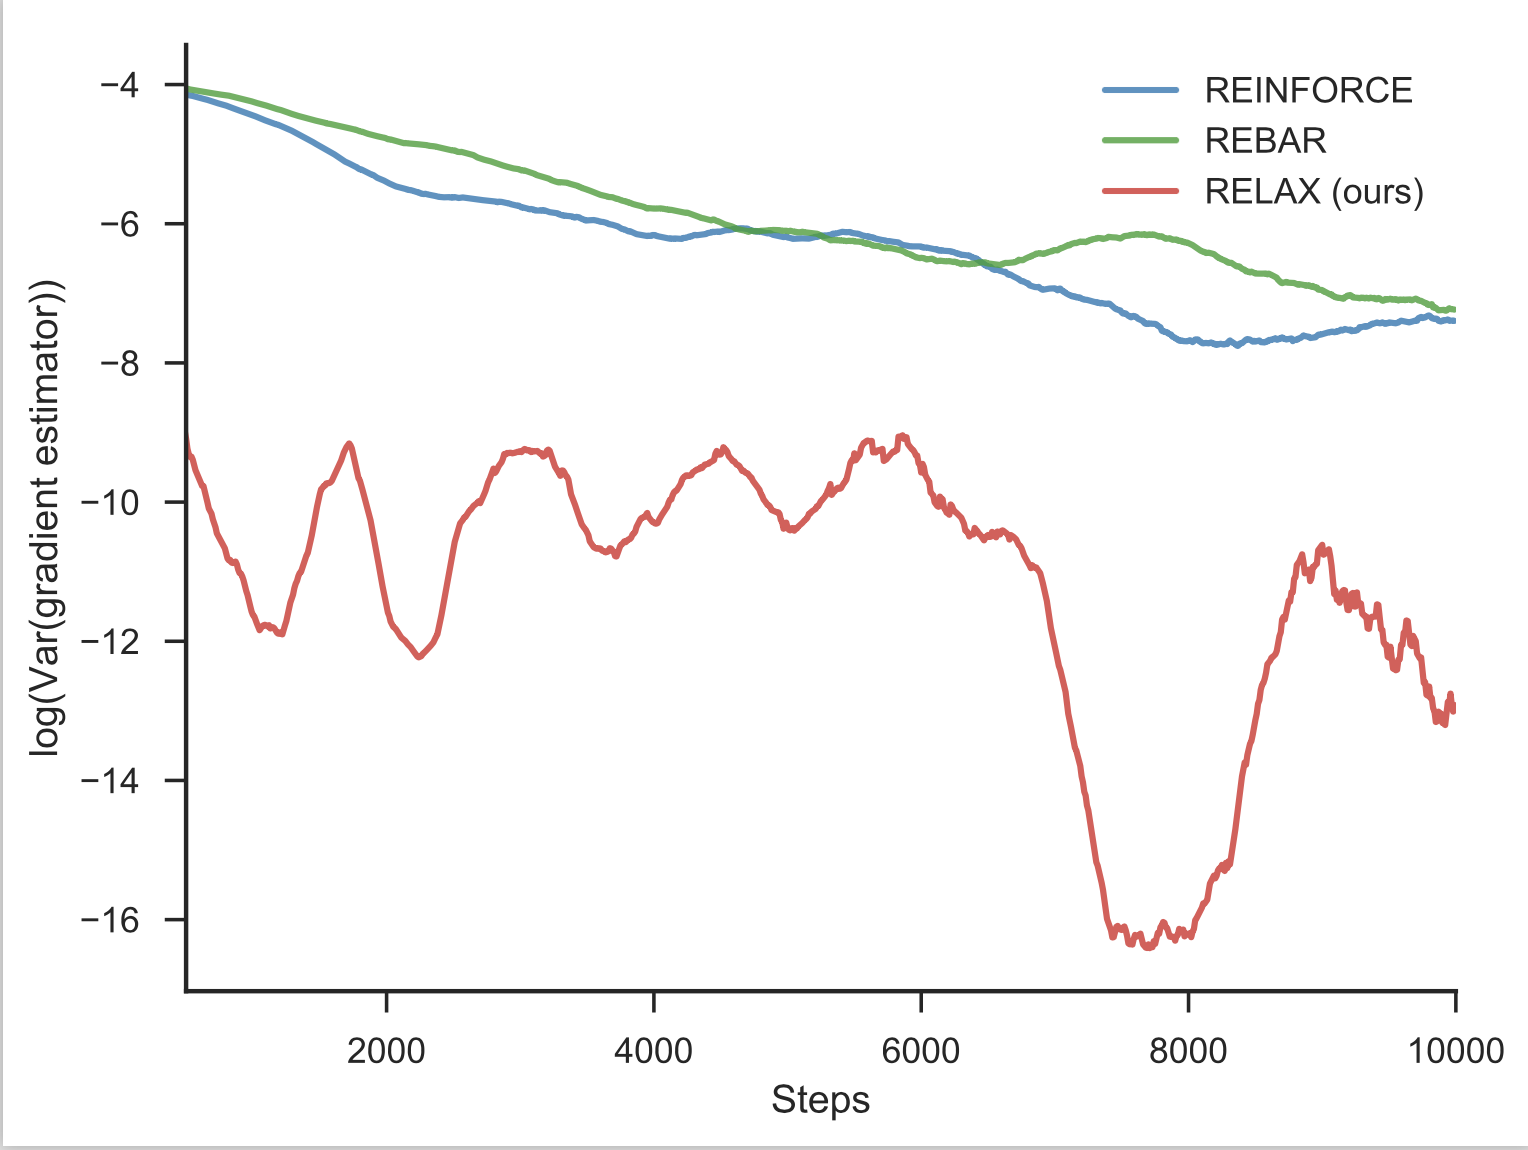
\includegraphics[width=.3\textwidth]{figures/variance}
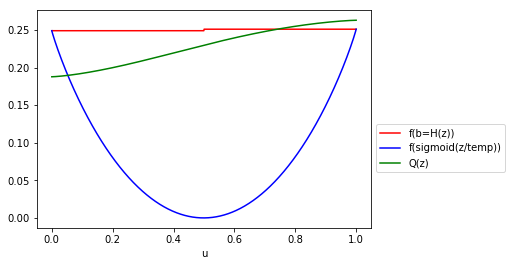
\includegraphics[width=.3\textwidth]{figures/learned_r}
\label{first figure}
\end{center}
\caption{
\emph{Left:} Training curves using different gradient estimators on a toy problem: {$\mathcal{L}(\theta) = \E_p(b|\theta) [ (b - 0.499)^2 ]$}
\emph{Centre:} Variance of each estimator's gradient.
\emph{Right:} The relaxation being used by REINFORCE (red), REBAR (blue), and the optimal relaxation (green).
}
\end{figure}


%Also: \citep{levine2016end}

\section{Background: Gradient estimators}

How can we choose the parameters of a distribution to maximize an expectation?
This problem comes up in reinforcement learning, where we must choose the parameters $\theta$ of a policy distribution $\pi(a|s, \theta)$ to maximize the expected reward $\mathbb{E}_{\tau \sim \pi} \left[ R \right]$ over state-action trajectories $\tau$.
It also comes up in fitting latent-variable models, when we wish to maximize the marginal probability ${p(x|\theta) = \sum p(x|z) p(z|\theta) = \mathbb{E}_{p(z|\theta)} \left[ p(x|z) \right]}$.
In this paper, we'll consider the general problem of optimizing
%
\begin{align}
\mathcal{L}(\theta)=\expectedLoss{}.
\end{align}
%
%Later, we will discuss the case when $\loss{}$ depends directly on $\theta$.

When the parameters $\theta$ are high-dimensional, gradient-based optimization is a appealing because it provides information about how to adjust each parameter individually.
Stochastic optimization is essential for scalablility, but is only guaranteed to converge to a fixed point of the original objective when the stochastic gradients $\hat g$ are unbiased, i.e. ${\mathbb{E} \left[ \hat g \right] = \PT \mathbb{E}_{p(b|\theta)} \left[ f(b) \right]}$~\citep{robbins1951stochastic}.

%Below we review past work in gradient estimation.
%There are a few general strategies for constructing unbiased gradient estimators:
How can we build unbiased, stochastic estimators of $\PT \mathcal{L}(\theta)$?
There are several standard methods:

\paragraph{The score-function gradient estimator}
One of the most generally-applicable gradient estimators is known as the score-function estimator, or REINFORCE~\citep{williams1992simple}:
%
\begin{align}
\hat g_\textnormal{reinforce} =  f \left( b \right) \PT \log p(b | \theta), \qquad b \sim p(b | \theta)
\end{align}
%
This estimator is unbiased, but in general has high variance.
Intuitively, this estimator is limited by the fact that it doesn't use any information about how $f$ depends on $b$, only on the final outcome $f(b)$.

\paragraph{The reparameterization trick}
When $f$ is continuous and differentiable, and the latent variables $b$ can be written as a deterministic, differentiable function of a random draw from a fixed distribution, the reparameterization trick \citep{williams1992simple, kingma2013autoencoding, rezende2014stochastic} creates a low-variance, unbiased gradient estimator by making the dependence of $b$ on $\theta$ explicit:
%
\begin{align}
%\hat g_\textnormal{reparam} = \frac{\partial f \left( b(\theta, \epsilon) \right)}{\partial \theta}, \qquad \epsilon \sim p(\epsilon)
\hat g_\textnormal{reparam}
= \PT f \left( b(\theta, \epsilon) \right)
= \frac{\partial f}{\partial b} \frac{\partial b(\theta, \epsilon)}{\partial \theta}, 
\qquad \epsilon \sim p(\epsilon) 
\end{align}
%
This gradient estimator is often used when training high-dimensional, continuous latent-variable models, such as variational autoencoders or GANs.
One intuition for why this gradient estimator is preferable to REINFORCE is that it depends on $\partial f / \partial b$, which exposes the dependence of $f$ on $b$.

\paragraph{Control variates}
Control variates are a general method for reducing the variance of a Monte Carlo estimator.
Given an estimator $g(b)$, a control variate is a function $\controlf(b)$ with a known mean $\mathbb{E}_{p(b)} [ \controlf ]$.
Subtracting the control variate from our estimator and adding its mean gives us a new estimator:
%
\begin{align}
\hat g_\textnormal{new}(b) = g(b) - \controlf(b) + \mathbb{E}_{p(b)}[\controlf(b)]
\end{align}
%
This new estimator has the same expectation as the old one:
%
\begin{align}
\mathbb{E}_{p(b)}\left[ g_\textnormal{new}(b) \right] 
= \mathbb{E}_{p(b)}\left[g(b) - \controlf(b) + \mathbb{E}_{p(b)} \left[ \controlf(b) \right] \right]
%= \mathbb{E}_{p(b)}\left[f(b) \right] - \mathbb{E}_{p(b)} \left[ \controlf(b) \right] + \mathbb{E}_{p(b)} \left[ \controlf(b) \right]
= \mathbb{E}_{p(b)}\left[ g(b) \right]
\end{align}
%
Importantly, the new estimator has lower variance than $g(b)$ if $\controlf(b)$ is positively correlated with $f(b)$.



\section{Gradient estimation with \LAX{} and \RELAX{}}
\label{lax section}
The reparameterization trick has become the favored method for gradient estimation recently but it is only applicable when $f$ is a known, differentiable function of continuous random variables. Similarly, for functions $f$ of discrete variables, methods involving continuous relaxations of discrete distributions such as concrete \cite{maddison2016concrete}, gumbel-softmax \cite{jang2016categorical}, and REBAR \cite{tucker2017rebar} have become popular. These methods also require that $f$ is known and differentiable with respect to its inputs. Moreover, they require that $f$ be computable at and behave predictably at inputs outside of the domain of the function. While these assumptions often hold, there are many problems of interest which make these approaches inapplicable. 

In this section, we introduce a gradient estimator for the expectation of a function $\PT \E_{p(b|\theta)}[f(b)]$. We make no assumptions about the structure of $f$ itself. This allows the estimator to be applied to a wide-range of applications with little or no modification. This estimator combines the score function estimator, the reparameterization trick, and control variates.
We obtain an unbiased estimator whose variance can potentially be as low as reparameterization-trick estimator, even when $f$ is not differentiable or not computable.

We begin with the case where $p(b|\theta)$ is a distribution over continuous random variables which is reparameterizable. We then handle the case where $p(b|\theta)$ is a distribution over discrete random variables. 

\subsection{The \LAX{} estimator for continuous random variables}

We begin with the score-function gradient estimator:
%
\begin{align}
\hat g_\textnormal{reinforce} =  f \left( b \right) \PT \log p(b | \theta), \qquad b \sim p(b | \theta)
\end{align}
%
Optimally, we would use the reparameterization trick but we do not assume that $f$ admits this.
Instead, we build a surrogate \emph{relaxation} of $f$ using a neural network $r_\phi$, and use the reparameterization trick on $r_\phi$ instead.
Using the fact that the score-function estimator and reparameterization estimator have the same expectation:
%
\begin{align}
\E_{p(\epsilon)} \left[ r_\phi ( b(\epsilon, \theta)) \PT \log p(b | \theta) \right] =
\E_{p(\epsilon)} \left[ \frac{\partial r_\phi}{\partial b} \frac{\partial b(\theta, \epsilon)}{\partial \theta} \right]
\end{align}
%

%We first consider the case where $b$ is a continuous random variable.% and then when $b$ is discrete.

%\subsection{The \LAX{} estimator -- continuous case} 
%\YW{The symbol $T$ usually refers to sufficient statistics. I don't think we should use it here for reparameterization. Also we should use a lower case letter.}
%We wish to compute $\PT\E_{p(b;\theta)}[f(b)]$ where $p(b;\theta)$ is a distribution with continuous support that admits a reparameterization $b = g_\theta(\epsilon)$, where $\epsilon \sim p(\epsilon)$.
%We assume that $f$ is a black-box, or involves operations such that $\PT f = 0$ almost everywhere or is not computable.
%\YW{This is the motivation for our following proposal. But I find it's not motivated enough.  It sounds like an assumption. But we're actually looking at this type of problem. I suggest motivate this more in the introduction paragraph, background section. List some examples of such $f$.} 
%Given the reparameterization, we can re-write this objective as an expectation over $\epsilon$ as  $\PT\E_{p(\epsilon)}[f(T(\epsilon, \theta)]$.

%Let $r_\phi$ be a differentiable function (such as a neural network) parametrized by $\phi$.
%By REINFORCE, we have $\PT\E_{p(b;\theta)}[r_\phi(b)] = \E_{p(b;\theta)}[r_\phi(b)\LP{b;\theta}]$.
%Hence, by adding and subtracting it, we have
%
%\begin{align}
%\PT\E_{p(b;\theta)}[f(b)] &= \E_{p(b;\theta)}\left[ \left[f(b) - r_\phi(b)\right]\cdot\LP{b;\theta}\right]+\PT\E_{p(b;\theta)}[r_\phi(b)]\nonumber\\
%&= \E_{p(\epsilon)} \left[ \left[f(g_\theta(\epsilon)) - r_\phi(g_\theta(\epsilon))\right]\cdot\LP{b} + \PT r(g_\theta(\epsilon))\right]\nonumber
%\end{align}
%
%Which allows us to define our estimator below as: 
%
We can simply add the score-function estimator and subtract the reparameterization estimator, to obtain:
%
\begin{align}
\label{eq:cont_est}
\hat g_\LAX = \left(f(b) -r_\phi(b)\right) \PT \log p(b|\theta) + \PT r_\phi(b) \qquad b = b(\theta, \epsilon), \epsilon \sim p(\epsilon).
\end{align}
%
%This estimator is unbiased for all choices of $r_\phi$. %, i.e $\E_\epsilon[g_\phi] = \PT\E_{p(b|\theta)}[f(b)]$. 
%A proof can be found in the appendix. 
This gives an unbiased estimator for any choice of $r_\phi$.

\begin{algorithm}[t]
\begin{algorithmic}
\Require $f(\cdot)$, $\log p(b|\theta)$, reparameterized sampler $b = T(\theta, \epsilon)$, neural network $r_\phi(\cdot)$
\While {not converged} 
	\State $\epsilon_{i} \sim p(\epsilon)$ \Comment Sample noise
	\State $b_i \leftarrow T(\epsilon_i, \theta)$ \Comment Compute input
	\State  $g_\theta \leftarrow \left[f(b_i) - r_{\phi}(b_i) \right] \nabla_\theta \log p + \nabla_\theta r(b_i)$ \Comment Estimate gradient
	\State  $g_\phi \leftarrow 2 g_\theta \frac{\partial g_\theta}{\partial \phi}$ \Comment Estimate gradient of variance of gradient
	\State $\theta \leftarrow \theta + \alpha_1 g_\theta$ \Comment Update parameters
	\State $\phi \leftarrow \phi + \alpha_2 g_\phi$ \Comment Update control variate
\EndWhile
\State \textbf{return} $\theta$ 
\end{algorithmic}
\label{discrete-relax}
\caption{\LAX{}: Optimizing parameters and a gradient control variate simultaneously.}
\end{algorithm}

\subsection{The \RELAX{} estimator for discrete random variables}
When $p(b|\theta)$ is a distribution over discrete random variables, more care must be taken. We assume that there exists a continuous, reparameterizable distribution $p(z|\theta)$ and a determanistic mapping $H(z)$ such that $H(z) = b \sim p(b|\theta)$ when $z \sim p(z|\theta)$. Examples of such distributions and functions can be found in the Appendix (section \ref{resample}). Most discrete distributions of interest fit into this formulation.

Introducing the parametric function $r_\phi$, we derive our estimator similarly to \cite{tucker2017rebar} with
%
\begin{align}
& \PT \expectedLoss{} \nonumber\\
&= \PT \E_{p(b|\theta)}\left[ f(b) \right] - \E_{p(z|\theta)}\left[ r_\phi(z) \right] + \PT\E_{p(z|\theta)}\left[ r_\phi(z) \right]\nonumber\\
&= \PT \E_{p(b|\theta)}\left[ f(b) - \E_{p(z|b, \theta)}\left[ r_\phi(z) \right]  \right] + \PT\E_{p(z|\theta)}\left[ r_\phi(z) \right]\nonumber\\
&= \E_{p(b|\theta)}\left[\left( f(b) - \E_{p(z|b, \theta)}\left[r_\phi(z) \right] \right)\PT \log p(b|\theta)  - \PT \E_{p(z|b, \theta)}\left[r_\phi(z) \right] \right] + \PT\E_{p(z|\theta)}\left[ r_\phi(z) \right]
%&= \E_{p(\epsilon, \hat{\epsilon})}\Big[\left( f(H(T(\epsilon, \theta))) - r_\phi(T(\epsilon, \theta))  \right) \PT \log p(H(T(\epsilon, \theta))|\theta) - \PT r_\phi(\hat{T}(\hat{\epsilon}, H(T(\epsilon, \theta)), \theta)) \Big]\nonumber\\
%&\qquad + \PT\E_{p(\epsilon)}\left[ r_\phi(T(\epsilon, \theta)) \right]
\end{align}
which allows us to define our estimator as
\begin{align}
\hat g_\textnormal{RELAX} = \left(f(b) - r_\phi(\hat{z})\right)\PT \log p(b|\theta) + \PT r_\phi(z) - \PT r_\phi (\tilde{z}) \\
\qquad b = H(z), z \sim p(z|\theta), \tilde{z} \sim p(z|b, \theta) \nonumber
\end{align}
%
which is also unbiased for any $r_\phi$. We note that the distribution $p(z|b,\theta)$ must also be reparameterizable. This is the case for Bernoulli and Categorical random variables. We demonstrate how to perform this conditional reparameterization in the Appendix (section \ref{resample}).


\subsection{Optimizing the gradient control variate with gradients}
Both presented estimators are unbiased for any choice of the function $r_\phi$, so the only remaining problem is to choose a $r_\phi$ that gives low variance to $\hat g_\LAX$ and $\hat g_\RELAX{}$.
How can we find a $\phi$ which gives our estimator low variance?
We simply optimize $r_\phi$ using stochastic gradient descent, at the same time as we optimize the parameters of our model or policy.

To optimize $r_\phi$, we require the gradient of the variance of our gradient estimator.
To estimate these gradients, we could simply differentiate through the empirical variance over each mini-batch.
Or, following \cite{tucker2017rebar}, we can construct an unbiased, single-sample estimator using the fact that our gradient estimator is unbiased. For any unbiased gradient estimator $\hat g$ with parameters $\phi$:
%
\begin{align}
\PPH \text{Variance}(\hat g)
= \PPH \E[\hat g^2] - \PPH \E[\hat g]^2
%= \PPH \E[\hat g^2] - \PPH \E_{p(b|\theta)}[f(b)]
= \PPH \E[\hat g^2]
= \E \left[ \PPH \hat g^2 \right]
= \E \left[ 2 \hat g \frac{\partial \hat g}{\partial \phi} \right].
\end{align}  % Do we need hats on these gs?  Or get rid of them elsewhere.
%
Thus, our estimator of the gradient of the variance of $\hat g$ is given by {$2 \hat g \frac{\partial \hat g}{\partial \phi}$}.

What is the form of the variance-minimizing $r_\phi$?
From inspection of the square of the estimator in \eqref{eq:cont_est} we can see that this loss encourages $r_\phi(b)$ to approximate $f(b)$, but with a weighting based on $\PT\log p(b)$.  % Todo: reword this awkward sentence.
Moreover, as $r_\phi \rightarrow f$ then $\hat g_\textnormal{\LAX} \rightarrow \PT r_\phi$.
Thus, this objective encourages a balance between the variance of the reparameterization estimator and the variance of the REINFORCE estimator. 

This method of directly minimizing the variance of the gradient estimator stands in contrast to other methods such as Q-Prop \cite{gu2016q} and advantage actor-critic \cite{mnih2016asynchronous}, which train the control variate to minimize the squared error $(f(b) - r_\phi(b))^2$.
Our algorithm, which jointly optimizes the parameters $\theta$ and the relaxation $r_\phi$ is given in Algorithm \ref{discrete-relax}.
%[Todo: talk about the variance of the gradient estimator of the variance of the gradient estimators?]

\subsection{Designing the control variate}
We have introduced a generic family of algorithms which produce unbiased and potentially low variance estimates of $\PT \E_{p(b|\theta)}[f(b)]$. Furthermore, we provide a tractable method to optimize the parameters of the control variate to minimize the variance of the estimator. The generality of this approach allows us to design our control variate $r_\phi$ in any way we please. This allows us to utilize any known structure that exists in $f$ to build a suitable control variate.

If, for example, $f$ is a known, differentiable, function of discrete random variables, we can utilize the concrete relaxation \cite{maddison2016concrete} and let $r_\phi(z) = f(\sigma_\lambda(z))$ in which case our estimator is exactly the REBAR estimator. We are also free to add a learned component to the concrete relaxation and let $r_\phi(z) = f(\sigma_\lambda(z)) + \hat{r}_\rho(z)$ where $\hat{r}_\rho$ is a neural network with parameters $\rho$. We have taken this approach in our experiments training discrete variational auto-encoders. If no information about $f$ is known, then we are also free to let $r_\phi$ be a generic function approximator such as a neural network. This is the approach we have taken in our reinforcement learning experiments. The variance-reduction objective introduced above allows us to use any differentiable, parametric function as our control variate. 


%\section{Conditional reparameterization}
%\label{conditional reparam section}
%To apply our method to discrete random variables, we incorporate a further refinement, based on a technique adapted from the REBAR method of \citet{tucker2017rebar}.
%First, we must introduce another 
%%
%
%A similar relaxation for the Bernoulli distribution has been developed as well (see Appendix for details)
%This gradient estimator is fairly effective in practice, but produces biased gradients, hindering its usage.
%Additionally, it is not clear how to set the temperature $\lambda$ and it is often treated as a hyperparameter.
%
%\paragraph{REBAR}
%REBAR gives unbiased estimates of the gradient of expectations of known functions of Bernoulli random variables.
%This method uses the REINFORCE estimator with a control variate.
%The control variate is derived from the original loss function evaluated at continuously-relaxed inputs \citep{maddison2016concrete, jang2016categorical}.
%The expectation of this control variate is estimated with low variance via the reparameterization trick. 
%
%\paragraph{Concrete relaxation}
%When $b$ is discrete and $f$ is known, one general approach is to differentiate a continuous relaxation of the discrete random variables.
%\cite{maddison2016concrete} and \cite{jang2016categorical} developed a differentiable relaxation of the categorical distribution, called the concrete distribution:
%
%\begin{align}
%\hat g_\textnormal{concrete} = \PT f \left( \sigma_\lambda ( \log \theta - \log(-\log u)) \right), \qquad u \sim \textnormal{uniform}[0, 1] 
%\end{align}
%
%where $\sigma_\lambda$ is the \texttt{softmax} function with temperature $\lambda$.
%
%Samples are drawn from $p(b|\theta)$ with a deterministic function of a continuous, reparameterizable random variable $z$. 
%
%\begin{align}
%z &:= g(u, \theta) = \log\frac{\theta}{1-\theta} + \log\frac{u}{1-u}, \qquad u \sim \text{uniform}[0,1]\nonumber\\
%b &:= \mathbb{I}(z>0)\nonumber
%\end{align}
%
%Thus, we can think of $p(b|\theta)$ as $\int p(b|z, \theta)p(z|\theta)dz$. The REBAR estimator is derived from this realization, noting:
%\begin{align}
%\PT \expectedLoss{} &= \PT \E_{p(b|\theta)}\left[ f(b) \right] - \PT\E_{p(z|\theta)}\left[ f(\sigma_\lambda(z) \right] + \PT\E_{p(z|\theta)}\left[ f(\sigma_\lambda(z) \right]\nonumber\\
%&= \PT \E_{p(b|\theta)}\left[ f(b) - \PT\E_{p(z|b, \theta)}\left[ f(\sigma_\lambda(z) \right]  \right] + \PT\E_{p(z|\theta)}\left[ f(\sigma_\lambda(z) \right]\nonumber\\
%&= \E_{p(b|\theta)}\left[\left( f(b) - \E_{p(z|b, \theta)}\left[ f(\sigma_\lambda(z) \right] \right)\PT \log p(b|\theta)  - \PT \E_{p(z|b, \theta)}\left[ f(\sigma_\lambda(z) \right] \right]\nonumber\\
%&\qquad + \PT\E_{p(z|\theta)}\left[ f(\sigma_\lambda(z) \right]\nonumber
%\end{align}
%
%where $\sigma_\lambda$ is the sigmoid function with temperature $\lambda$.
%The REBAR estimator is the single-sample monte-carlo estimator derived from the last line above.
%The REBAR estimator is computed as:
%\begin{align}
%\hat g_\textnormal{REBAR} = \left(f(b) - f(\sigma_\lambda(z)\right)\PT \log p(b|\theta) + \PT f(\sigma_\lambda(z)) - \PT f(\sigma_\lambda(\tilde{z}))\nonumber\\
%z \sim p(z|\theta), \tilde{z} \sim p(z|b, \theta), b = \mathbb{I}(z>0)\nonumber
%\end{align}
%Details of how to sample from $p(z|b, \theta)$ as well as an extension to categorical random variables can be found in the Appendix.
%\cite{tucker2017rebar} also introduced a way to optimize the temperature parameter $\lambda$ via gradient decent to minimize the variance of the estimator. 



%In the case where $p(b|\theta)$ is a distribution over discrete variables, a few more details arise.
%In this section, we first review the technique of concrete relaxation introduced in \cite{maddison2016concrete} and \cite{jang2016categorical}. 
%Inspired by REBAR \citet{tucker2017rebar}, we propose a more general family of gradient estimators called \RELAX{} for discrete variables. 

%We mainly consider the most commonly used discrete distribution, the Categorical distribution (which includes Bernoulli distribution as a special case).
%A well-known approach to obtain a sample from a Categorical distribution with probability vector $\theta = \{\theta_i\}_1^k$ is by
%\begin{align}
%z &= \log\theta - \log(-\log u),\qquad u \sim \text{uniform}[0,1]^k\nonumber \\
%b &= H(z), \nonumber
%\end{align}
%where $H(\cdot)$ is the \texttt{argmax} function. Inspired by REBAR \citet{tucker2017rebar}, we write $p(z|\theta)$ as $\int p(z|b, \theta)p(b|\theta)db$. Note that if $p(z|\theta)$ and $p(z|b, \theta)$ are reparameterizable, i.e., there exists $\hat{T}$ such that $\hat{T}(\hat{\epsilon}, b, \theta) = \hat{z} \sim p(z|b, \theta)$. See Appendix for details on sampling from $p(z|b, \theta)$ in both the Bernoulli and Categorical cases.
%As in \LAX{}, we let $r_\phi$ be an differentiable function. Now we derive our estimator as follows,
%
%\begin{align}
%\PT \expectedLoss{} &= \PT \E_{p(b|\theta)}\left[ f(b) \right] - \E_{p(z|\theta)}\left[ r_\phi(z) \right] + \PT\E_{p(z|\theta)}\left[ r_\phi(z) \right]\nonumber\\
%&= \PT \E_{p(b|\theta)}\left[ f(b) - \E_{p(z|b, \theta)}\left[ r_\phi(z) \right]  \right] + \PT\E_{p(z|\theta)}\left[ r_\phi(z) \right]\nonumber\\
%&= \E_{p(b|\theta)}\left[\left( f(b) - \E_{p(z|b, \theta)}\left[r_\phi(z) \right] \right)\PT \log p(b|\theta)  - \PT \E_{p(z|b, \theta)}\left[r_\phi(z) \right] \right]\nonumber\\
%&\qquad + \PT\E_{p(z|\theta)}\left[ r_\phi(z) \right]\nonumber\\
%&= \E_{p(\epsilon, \hat{\epsilon})}\Big[\left( f(H(T(\epsilon, \theta))) - r_\phi(T(\epsilon, \theta))  \right) \PT \log p(H(T(\epsilon, \theta))|\theta) \nonumber\\
%&\qquad\qquad\qquad - \PT r_\phi(\hat{T}(\hat{\epsilon}, H(T(\epsilon, \theta)), \theta)) \Big]\nonumber\\
%&\qquad + \PT\E_{p(\epsilon)}\left[ r_\phi(T(\epsilon, \theta)) \right]\nonumber
%\end{align}
%
%which allows us to define our estimator as
%
%\begin{align}
%\hat g_\textnormal{RELAX} = \left(f(b) -r_\phi(\hat{z})\right)\PT \log p(b|\theta) + \PT r_\phi(z) - \PT r_\phi (\tilde{z}) \nonumber\\
%\qquad b = H(z), z \sim p(z|\theta), \tilde{z} \sim p(z|b, \theta)
%\end{align}
%
%This estimator is also unbiased i.e $E_{\epsilon, \hat{\epsilon}}[g_\phi] = \PT\E_{p(b|\theta)}[f(b)]$.
%Therefore we can take the advantage of reparameterization to further reduce the variance of the estimator.



\section{Reinforcement Learning}
Reinforcement learning is strong motivating problem for methods similar to ours.
In reinforcement learning we seek to optimize the parameters of a policy distribution $\pi(a|s;\phi)$ to maximize the discounted sum of future rewards given that policy $\mathbb{E}_{\pi(\phi)}[\sum_{t=1}^{\infty} \gamma^{t-1} r_t]$ 
%\YW{add discounting factor into the formulation. You can refer to my paper or any standard RL paper and see how these things are defined.}.
We can view the sum of future rewards as a black-box function of state-action trajectories $\tau$ sampled from our policy.
Thus, as before we have reduced the problem to that of estimating $\frac{\partial \mathbb{E}_{\tau}[f(\tau)]}{\partial \phi}$ which is the standard policy gradient algorithm \cite{sutton2000policy}. 

We seek to compute $$\frac{\partial \E_\tau[R]}{\partial \theta} = \E\Big[\sum_{t=1}^T \LL{t} \sum_{t'=t}^T r_t\Big]$$ but the estimator on the right hand side can have potentially high variance. Instead, we typically compute
$$\frac{\partial \E_\tau[R]}{\partial \theta} = \E_\tau\Big[\sum_{t=1}^T \LL{t} [(\sum_{t'=t}^T r_{t'}) - b(s_t)]\Big]$$
Where $b(s_t)$ is an estimate of the state-value function, $b(s) \approx V^\pi(s) = \E_{\tau}[R|s_1=s].$
This is unbiased for any choice of $b$ since $b$ does not depend on $a_t$. 

\subsubsection{Reinforcement learning with \LAX{} and \RELAX{}}
We now describe how we apply \LAX{} and \RELAX{} estimators in the RL setting.
In the case of RL, $b$ is $\tau$, which denotes a series of actions and states $[s_1, a_1, s_2, a_2, ..., s_T, a_T]$, and the function $f$ refers to the underlying MDP, which maps $\tau$ to the sum of discounted reward, $R = \sum_{t=1}^T \gamma^t r_t$ with discount factor $\gamma$. 

We show the continuous case, and leave the discrete case to Appendix.
We assume $\pi(a_t|s_t)$ is reparametrizable meaning that we can write $a_t = g_\theta(\epsilon,s_t)$, where $\epsilon$ does not depend on $\theta$.
We again introduce a new differentiable function $r_\phi(a,s)$, and it's a function of the action and the state pair.
We observe that $\forall t$, we have (see details in Appendix \ref{}) $$\E_{p(\tau)}\Big[\LL{t} r_\phi(a_t, s_t)\Big] = \E_{p(a_{1:t-1},s_{1:t})}\Big[\frac{\partial}{\partial\theta}\E_{\pi(a_t|s_t, \theta)}\Big[r_\phi(a_t, s_t)\Big]\Big]$$ 
Then by adding and subtracting the same term, we have
\begin{align*}
\PT\E_{p(\tau)}[f(\tau)] &= \E_{p(\tau)}\left[f(\tau)\cdot\LP{\tau;\theta}\right]-\sum_t\E_{p(\tau)}\Big[\LL{t} r_\phi(a_t, s_t)\Big]+\\&\sum_t \E_{p(a_{1:t-1},s_{1:t})}\Big[\frac{\partial}{\partial\theta}\E_{\pi(a_t|s_t, \theta)}\Big[r_\phi(a_t,s_t)\Big]\Big]\nonumber\\
&= \E_{p(\tau)}\left[ \sum_{t=1}^T \LL{t}\left(\sum_{t'=t}^T r_{t'} - r_\phi(a_t,s_t)\right)\right]+\sum_t \E_{p(a_{1:t-1},s_{1:t})}\Big[\E_{p(\epsilon_t)}\Big[\frac{\partial}{\partial\theta}r_\phi(g_\theta(\epsilon_t,s_t), s_t)\Big]\Big]\nonumber\\
&= \E_{p(\tau)}\left[ \sum_{t=1}^T \LL{t}\left(\sum_{t'=t}^T r_{t'} - r_\phi(a_t,s_t)\right)+\frac{\partial}{\partial\theta}r_\phi(g_\theta(\epsilon_t,s_t), s_t)\right]\nonumber
\end{align*}

Hence our estimate is defined as: 
\begin{align}
\label{eq:rl_est}
\hat g_\LAX^{\RL} = \sum_{t=1}^T \LL{t}\left(\sum_{t'=t}^T r_{t'} - r_\phi(a_t,s_t)\right)+\frac{\partial}{\partial\theta}r_\phi(g_\theta(\epsilon_t,s_t), s_t), \\ a_t =g_\theta(\epsilon_t,s_t) \qquad \epsilon_t \sim p(\epsilon_t)\nonumber.
\end{align}


\section{Related work}
%\YW{For this section we can focus on comparisons to REBAR, because it is the most related one which might also raise most questions. We can briefly mention previous methods for doing discrete variables. We should also mention Q-prop.}
The recently-developed REBAR method \citep{tucker2017rebar} is the work most related to ours.
REBAR estimates the gradient of expectations of functions of Bernoulli random variables.
This method uses the REINFORCE estimator with a control variate.
The control variate is derived from the original loss function evaluated at continuously-relaxed inputs \citep{maddison2016concrete, jang2016categorical}.
The expectation of this control variate is estimated with low variance via the reparameterization trick. The REBAR estimator can been seen as a special case of the RELAX estimator when $r_\phi(z) = f(\sigma_\lambda(z))$.
\label{limitations}
%While the above approaches have greatly broadened the scope of functions whose derivatives we can approximate, there still exist a number of factors limiting their application to many problems of interest.

%The bias induced by the concrete relaxation can lead to convergence at unsuitable optima or no convergence at all.
%REBAR alleviates these issues by using the relaxation as a control variate for the estimator instead of using it as the estimator itself.
Unfortunately, REBAR and concrete require the function being optimized, whose input is only defined at discrete inputs, to also accept continuous inputs, be differentiable w.r.t. those inputs, and behave predictably with respect to those continuous inputs.
While often true, these are strong assumptions to make.
Furthermore, REBAR and concrete require that the function being optimized is known. 
This makes REBAR and the concrete relaxation inapplicable for optimizing black-box functions, as in reinforcement learning settings where the reward is an unknown function of the environment.

In contrast, \LAX{} and \RELAX{} can be used in these settings.
\LAX{} and \RELAX{} only require that we can query the function being optimized, and can sample from and differentiate $p(b|\theta)$.

Can \RELAX{} be used to optimize deterministic black-box functions?
The answer is yes, with the caveat that one must introduce stochasticity to the inputs.
Thus, \RELAX{} is most suitable for problems where one is already optimizing a distribution over inputs, such as in inference or reinforcement learning.
% Note that most optimal policies are deterministic?

There has been a great deal of other recent work in the area of gradient estimation. \citet{miller2017reducing} reduce the variance of reparameterization gradients in an orthogonal way to ours by approximating the gradient-generating procedure with a simple model and using that model as a control variate. NVIL~\citep{mnih2014neural}, VIMCO~\citep{mnih2016variational} provide reduced variance gradient estimation in the special case of discrete latent variable models and discrete latent variable models with monte-carlo objectives. \citet{salimans2017evolution} estimate gradients using a form of finite differences, evaluating hundreds of different parameter values in pararallel to construct a gradient estimator.
In contrast, our method is a simple-sample estimator.

%As gradient estimators become more complex, checking their unbiasedness numerically becomes difficult.
%The automatic theorem-proving-based unbiasedness checker developed by \citet{selsam2017developing} may become relevant to this line of research.


\citet{staines2012variational} address the general problem of developing gradient estimators for deterministic black-box functions or discrete optimization.
They introduce a sampling distribution, and optimize an objective similar to ours.
\citet{wierstra2014natural} also introduce a sampling distribution to build a gradient estimator, and consider optimizing the sampling distribution.

In the reinforcement learning setting, the work most similar to ours is $Q$-prop \cite{haarnoja2017reinforcement}.
Like our method, $Q$-prop reduces the variance of the policy gradient with an learned, action-dependent control variate whose expectation is approximated via a monte-carlo sample from a taylor series expansion of the control variate.
Unlike our method, their control variate is trained off-policy. While our method is applicable in both the continuous and discrete action domain, $Q$-prop is only applicable in environments with continuous actions. We are interested in the potential of training our control variate off-policy, but we leave that for further work. 

%\citet{asadi2017mean} reduce the variance of actor-critic gradient estimates by simply summing over all possible actions.

%\par{Generalized Reparameterization Gradients}
%REBAR and the generalization in this paper uses a mixture of score function and reparameterization gradients.
%A recent paper by \cite{ruiz2016generalized} unifies these two gradient estimators as the generalized reparameterization gradient (GRG).
%This framework can help disentangle the various components of generalized REBAR.

%REBAR innovation as further decomposition the correction term into secondary reparameterization components
%note this is a recursive application of the principles of GRG
%observe that the GRG suggests this recursive application to components of an estimator
%propose that other estimators could be similarly recursively decomposed?


\section{Applications}
\label{Applications}
We demonstrate the effectiveness of our estimator on a number of challenging optimization problems. Following \cite{tucker2017rebar} we begin with a simple toy example to illuminate the potential of our method and then continue to the more relevant problems of optimizing binary VAE's and reinforcement learning.

\subsection{Toy Experiment}
We seek to minimize $\mathbb{E}_{p(b|\theta)}[(b - t)^2]$ as a function of the parameter $\theta$ where $p(b|\theta) = \mathtt{Bernoulli}(b|\theta)$. \cite{tucker2017rebar} set the target $t = .45$.
We focus on the more challenging case where $t = .499$.
With this setting of the target, REBAR and competing methods suffer from high variance and are unable to discover the optimal solution $\theta = 0$.

The fixed Concrete relaxation of REBAR is unable to produce a gradient whose signal outweighs the sample noise and is therefore unable to solve this problem noticeably faster than REINFORCE.
Figure \ref{fig:toy_var} plots the learned relaxations for a fixed value of $\theta$.

It can be seen that RELAX learns a relaxation whose derivative points in the direction of decreased loss for all values of reparameterization noise $u$, whereas REBAR's fixed relaxation only does so for values of $u > t$.


\subsection{Discrete Variational Autoencoder}
As in \citep{tucker2017rebar}, we benchmark the RELAX estimator on the task of training a variational autoencoder \citep{kingma2013autoencoding, rezende2014stochastic} where all random variables are Bernoulli taking values in $\{-1, 1\}$.
As in \cite{tucker2017rebar}, we compare training the variational lower-bound across the MNIST and Omniglot~\citep{lake2015human} datasets.
As in \cite{tucker2017rebar} we test models with 1 and 2 layers of 200 Bernoulli random variables with linear mappings between them. 

In the one layer models we optimize the ELBO $$\mathcal{L}(\theta) = \E_{q(b|x)}[\log p(x|b) + \log p(b) - \log q(b|x)]$$ where $q(b_1|x) = \sigma(x\cdot W_q + \beta_q)$ and $p(x| b_1) = \sigma(b_1\cdot W_p + \beta_p)$ with weight matrices $W$ and biases $\beta$. The parameters of the prior $p(b)$ are also learned. Details of the two layer model can be found in the Appendix (section \ref{app_disc_vae}).

%them and a model with 1 layer of Bernoulli random variables with non-linear mappings between layers.

To take advantage of the available structure in the loss function, we choose the form of our control variate to be $$ r_\phi(z) = \hat{r}_\rho(z) + f(\sigma_\lambda(z))$$ where $\hat{r}_\rho$ is a neural network with parameters $\rho$ and $f(\sigma_\lambda(z))$ is the discrete loss function (the evidence lower-bound) evaluated at continuously relaxed inputs as in REBAR.  
%We found that due to the complicated structure of the loss function, the RELAX estimator performed worse than REBAR. Instead we add a learned relaxation to REBAR's control variate which we denote relaxed-REBAR.
%Our estimator takes the form of \eqref{eq:RELAX} with $$\bar \relaxed(z) = \relaxed(z) + f(\sigma_\lambda(z))$$ where $\relaxed(z)$ is a learned neural network and $f(\sigma_\lambda(z))$ is the Concrete relaxation of REBAR with temperature parameter $\lambda$.

We compare against the strong baseline of REBAR \cite{tucker2017rebar}. In all experiments, we observed that the learned control variate improved the training and validation performance as well as increased the rate of convergence. 

\begin{table}[h]
\begin{center}
\begin{tabular}{l c c c c c} 
& NVIL & MuProp & REBAR & REBAR & RELAX \\
\textbf{MNIST} & & & \citet{tucker2017rebar} & ours & \\\midrule
%Nonlinear      & $-102.2$ & $-101.5$ & -101.1  &  -81.01 &  \textbf{-78.13} \\
Linear 1 layer  & $-112.5$ & $-111.7$ & -111.6 & -111.6 & \textbf{-111.20} \\ 
Linear 2 Layer  & $-99.6$ & $-99.07$ & -98.8  & -98.22 & \textbf{-98.00} \\\\
\textbf{Omniglot}\\ \midrule
%Nonlinear      & $-110.4$  & $-109.58$ & -108.72  & -62.28 & \textbf{-58.55} \\
Linear 1 layer & $-117.44$ & $-117.09$ & -116.83  & -116.63 & \textbf{-116.57} \\ 
Linear 2 Layer & $-109.98$ & $-109.55$ & -108.71  & -108.71 & \textbf{-108.54}
\end{tabular}
\end{center}
\label{tab:vae_tr}
\caption{Best obtained training objective.}
\end{table}

\begin{table}[h]
\begin{center}
\begin{tabular}{l c c} 
               & REBAR & RELAX \\
\textbf{MNIST} & ours  & \\\midrule

Linear 1 layer  & -114.32 & \textbf{-113.62} \\ 
Linear 2 Layer  & -101.20 & \textbf{-100.85} \\\\
\textbf{Omniglot}\\ \midrule

Linear 1 layer & -122.44 & \textbf{-122.11} \\ 
Linear 2 Layer & -115.83 & \textbf{-115.42}
\end{tabular}
\end{center}
\label{tab:vae_val}
\caption{Best obtained validation objective.}
\end{table}

%In \citep{tucker2017rebar}, a separate REBAR estimator was used to estimate the gradients of each model parameter (each weight matrix and bias vector).
%To apply our estimator to this formulation, we would need to learn a separate relaxation for each model parameter.
%To get around this, we use our gradient estimator to approximate $g_\phi \approx \PT \E_{q(b|\theta)}[f(b)]$ where $x\cdot W = \theta$ is the parameters of the Bernoulli latent variables, $W$ is our layer's weight matrix. We then obtain an estimate of $\PP{W} \E_{q(b|\theta)}[f(b)] = g_\phi\cdot \frac{\partial \theta}{\partial W}$. We note this gives us unbiased gradients because 
%\begin{align}
%\E_\epsilon[g_\phi(\epsilon) \cdot \frac{\partial \theta}{\partial W}] = \E_\epsilon[g_\phi(\epsilon)] \cdot \frac{\partial \theta}{\partial W} =  \PT \E_{q(b|\theta)}[f(b)] \cdot \frac{\partial \theta}{\partial W} = 
%\frac{\partial}{\partial W} \E_{q(b|\theta)}[f(b)]
%\end{align} 

%To provide a fair comparison, we re-implemented REBAR in this way (denoted REBAR-ours in table~\ref{tab:vae}).
%We believe this explains the large difference in performance between our implementation and that of \citep{tucker2017rebar} for the nonlinear models since there are 3 layers of parameters that all share the same gradient estimator.
%In the linear models, each layer has its own gradient estimator making our implementation closer to that of \citep{tucker2017rebar}.
To obtain training curves we created our own implementation of REBAR. The scores of this model are denoted ``REBAR ours'' in the following tables. We obtained identical or slightly improved performance with our implementation.

While we obtained a modest improvement in training and validation scores (tables \ref{tab:vae_tr} and \ref{tab:vae_val}), the most notable improvement provided by RELAX is in its rate of convergence. Training curves for all models can be seen in figures \ref{fig:vae_mnist} and \ref{fig:vae_omni}. In table \ref{tab:vae_epochs} we compare the number of training epochs that are required to match the best validation score of REBAR. In all experiments, RELAX provides a large increase in rate of convergence. 

\begin{figure}[h]
\begin{center}
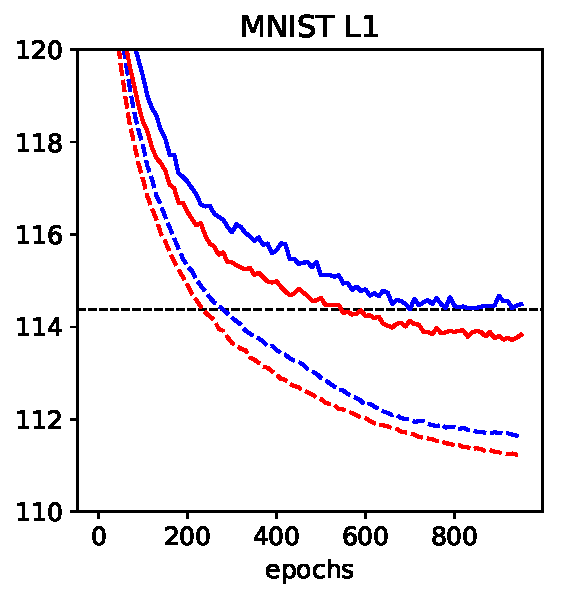
\includegraphics[width=.4\textwidth]{figures/MNIST_L1}
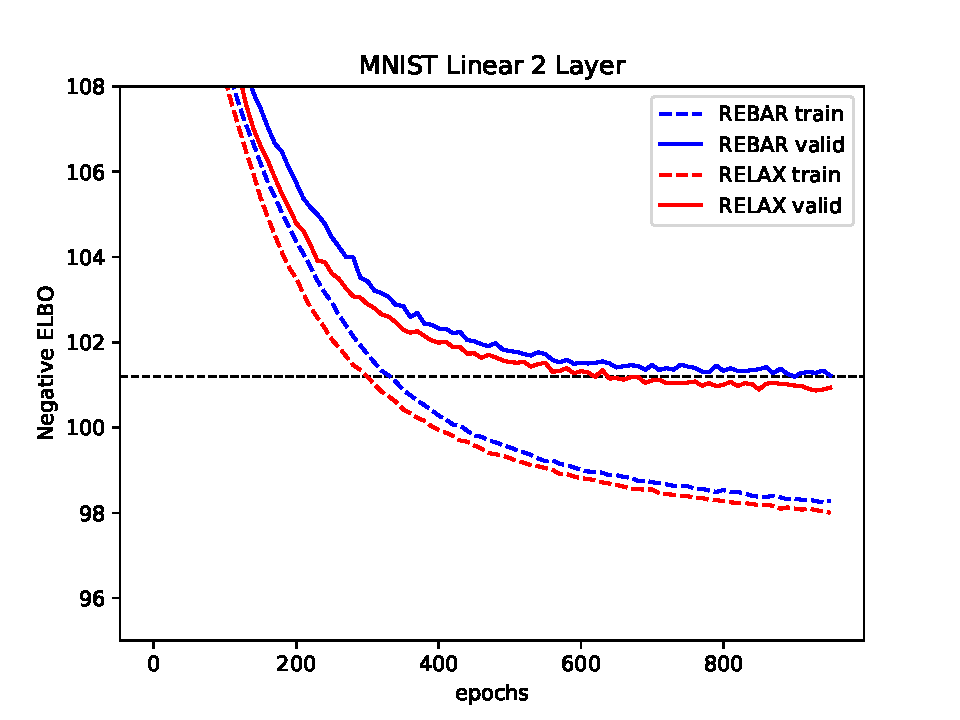
\includegraphics[width=.4\textwidth]{figures/MNIST_L2}
\label{fig:vae_mnist}
\end{center}
\caption{Training curves on MNIST. The horizontal dashed line indicates the lowest validation error obtained by REBAR.}
\end{figure}

\begin{figure}[h]
\begin{center}
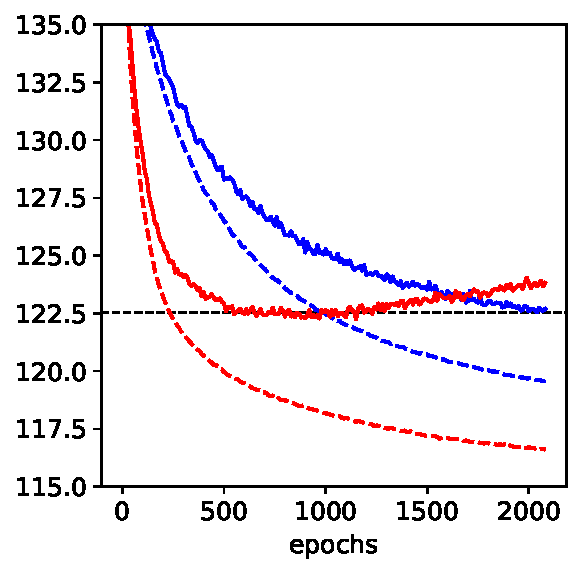
\includegraphics[width=.4\textwidth]{figures/OMNIGLOT_L1}
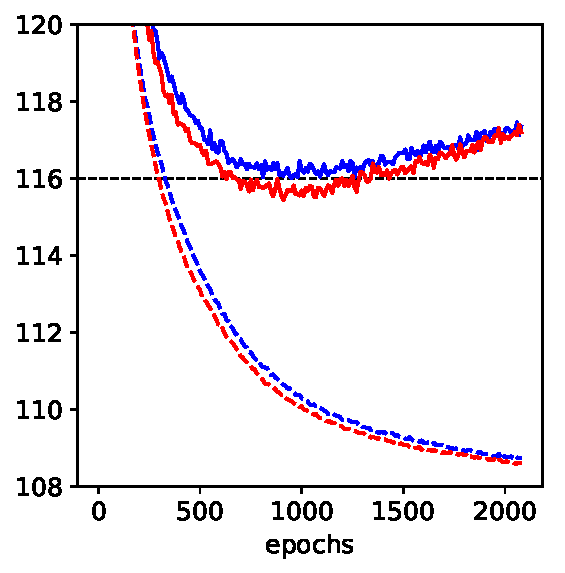
\includegraphics[width=.4\textwidth]{figures/OMNIGLOT_L2}
\label{fig:vae_omni}
\end{center}
\caption{Training curves on OMNIGLOT. The horizontal dashed line indicates the lowest validation score obtained by REBAR.}
\end{figure}

\begin{table}[h]
\begin{center}
\begin{tabular}{l c c} 
               & REBAR & RELAX \\
\textbf{MNIST} & ours  & \\\midrule

Linear 1 layer  & 857 & \textbf{531} \\ 
Linear 2 Layer  & 900 & \textbf{620} \\\\
\textbf{Omniglot}\\ \midrule

Linear 1 layer & 2086 & \textbf{566} \\ 
Linear 2 Layer & 1027 & \textbf{673}
\end{tabular}
\end{center}
\label{tab:vae_epochs}
\caption{Epochs needed to achieve REBAR's best validation score.}
\end{table}



\subsection{Reinforcement Learning}
We test our approach on a few simple reinforcement learning environments with discrete and continuous actions.
We use the \RELAX{} and \LAX{} estimators for discerete and continuous actions, respectively. We compare with the advantage actor-critic algorithm~\cite{sutton2000policy} as a baseline.
In all experiments we utilized the same learning rate for the policy network for RELAX and A2C so differences in performance depended solely on the control variate used. 

To compare these approaches in the most illustrative setting possible we do not use any reward bootstrapping in either model. After each episode terminates, we generate the discounted reward for each time-step, treat the episode as a single batch of data, and perform one step of gradient decent. We are aware that better results could be obtained with bootstrapping and larger batch sizes but we wanted to work in the highest possible variance setting to demonstrate the variance reduction capabilities of our approach.

%We test our alrgorithm on the Cart-Pole and Lunar-Lander environments from the OpenAI Gym~\cite{1606.01540}.
%We run the Cart-Pole and Lunar-Lander environments for 250 and 1000 episodes, respectively and plot reward and the log-variance of the policy gradients in figure~X.

\subsubsection{Discrete Experiments}
We test our approach in the discrete action domains of the CartPole and LunarLander as provided by the OpenAI gym~\cite{1606.01540}. For all models, the policy and control variate were both neural networks with 2 layers of 10 units using the ReLU nonlinearity. We first tuned the learning rate using the baseline A2C then ran \RELAX{} with the same learning rate. 
In both domains we observe improved performance and sample efficiency using our method. Again, we are aware that improved results could be obtained by further tuning the learning rate for \RELAX{} but we wanted to illustrate the improvement provided solely by the improved control variate. 

\paragraph{Experimental Details}
We estimate the policy gradient using a single Monte Carlo sample produced from a one episode roll-out of the current policy.
We note that improved performance could be achieved by using more samples, but we intended to test our model in the highest-possible variance setting. 
In all experiments both the policy and control variate were two layer neural networks with RELU non-linearities. Each intermediate layer's output had dimension 10. We searched over two hyper-parameters; the global learning rate and the scaling on the loss from the control variate or value function. For each we tested values in $[.01, .003, .001]$. between our model and the baseline and the learning rates were also constant across tests making it that all improvements derive from having a lower variance estimate of the policy gradient. Presented results are obtained by averaging over 5 runs with different random seeds. We run the CartPole and LunarLander for $250,000$ and $5,000,000$ time-steps respectively. 

\begin{table}[h]
\begin{center}
\begin{tabular}{l c c} 
\textbf{CartPole} & A2C & RELAX \\\midrule
Episodes until solve      & $1152 \pm 90$ & $\bm{472 \pm 114}$ \\\\
\textbf{LunarLander}\\ \midrule
Episodes until solve & $10703 \pm 4087$ & $\bm{5156.8 \pm 794.9}$ 
\end{tabular}
\end{center}
\label{tab:vae}
\caption{Mean Episodes to Solve. CartPole is considered solved if the agent receives an average reward over $195$ in the last $100$ Episodes. LunarLander is considered solved if the agent receives an average reward over $200$ in the last $100$ frames.}
\end{table}
% cartpole epsidoes to solve, this result looks better than episodes
% Best Models      & $81018 \pm 15405$ & $45729 \pm 16294$ \\\\

\begin{figure}[h]
\begin{center}
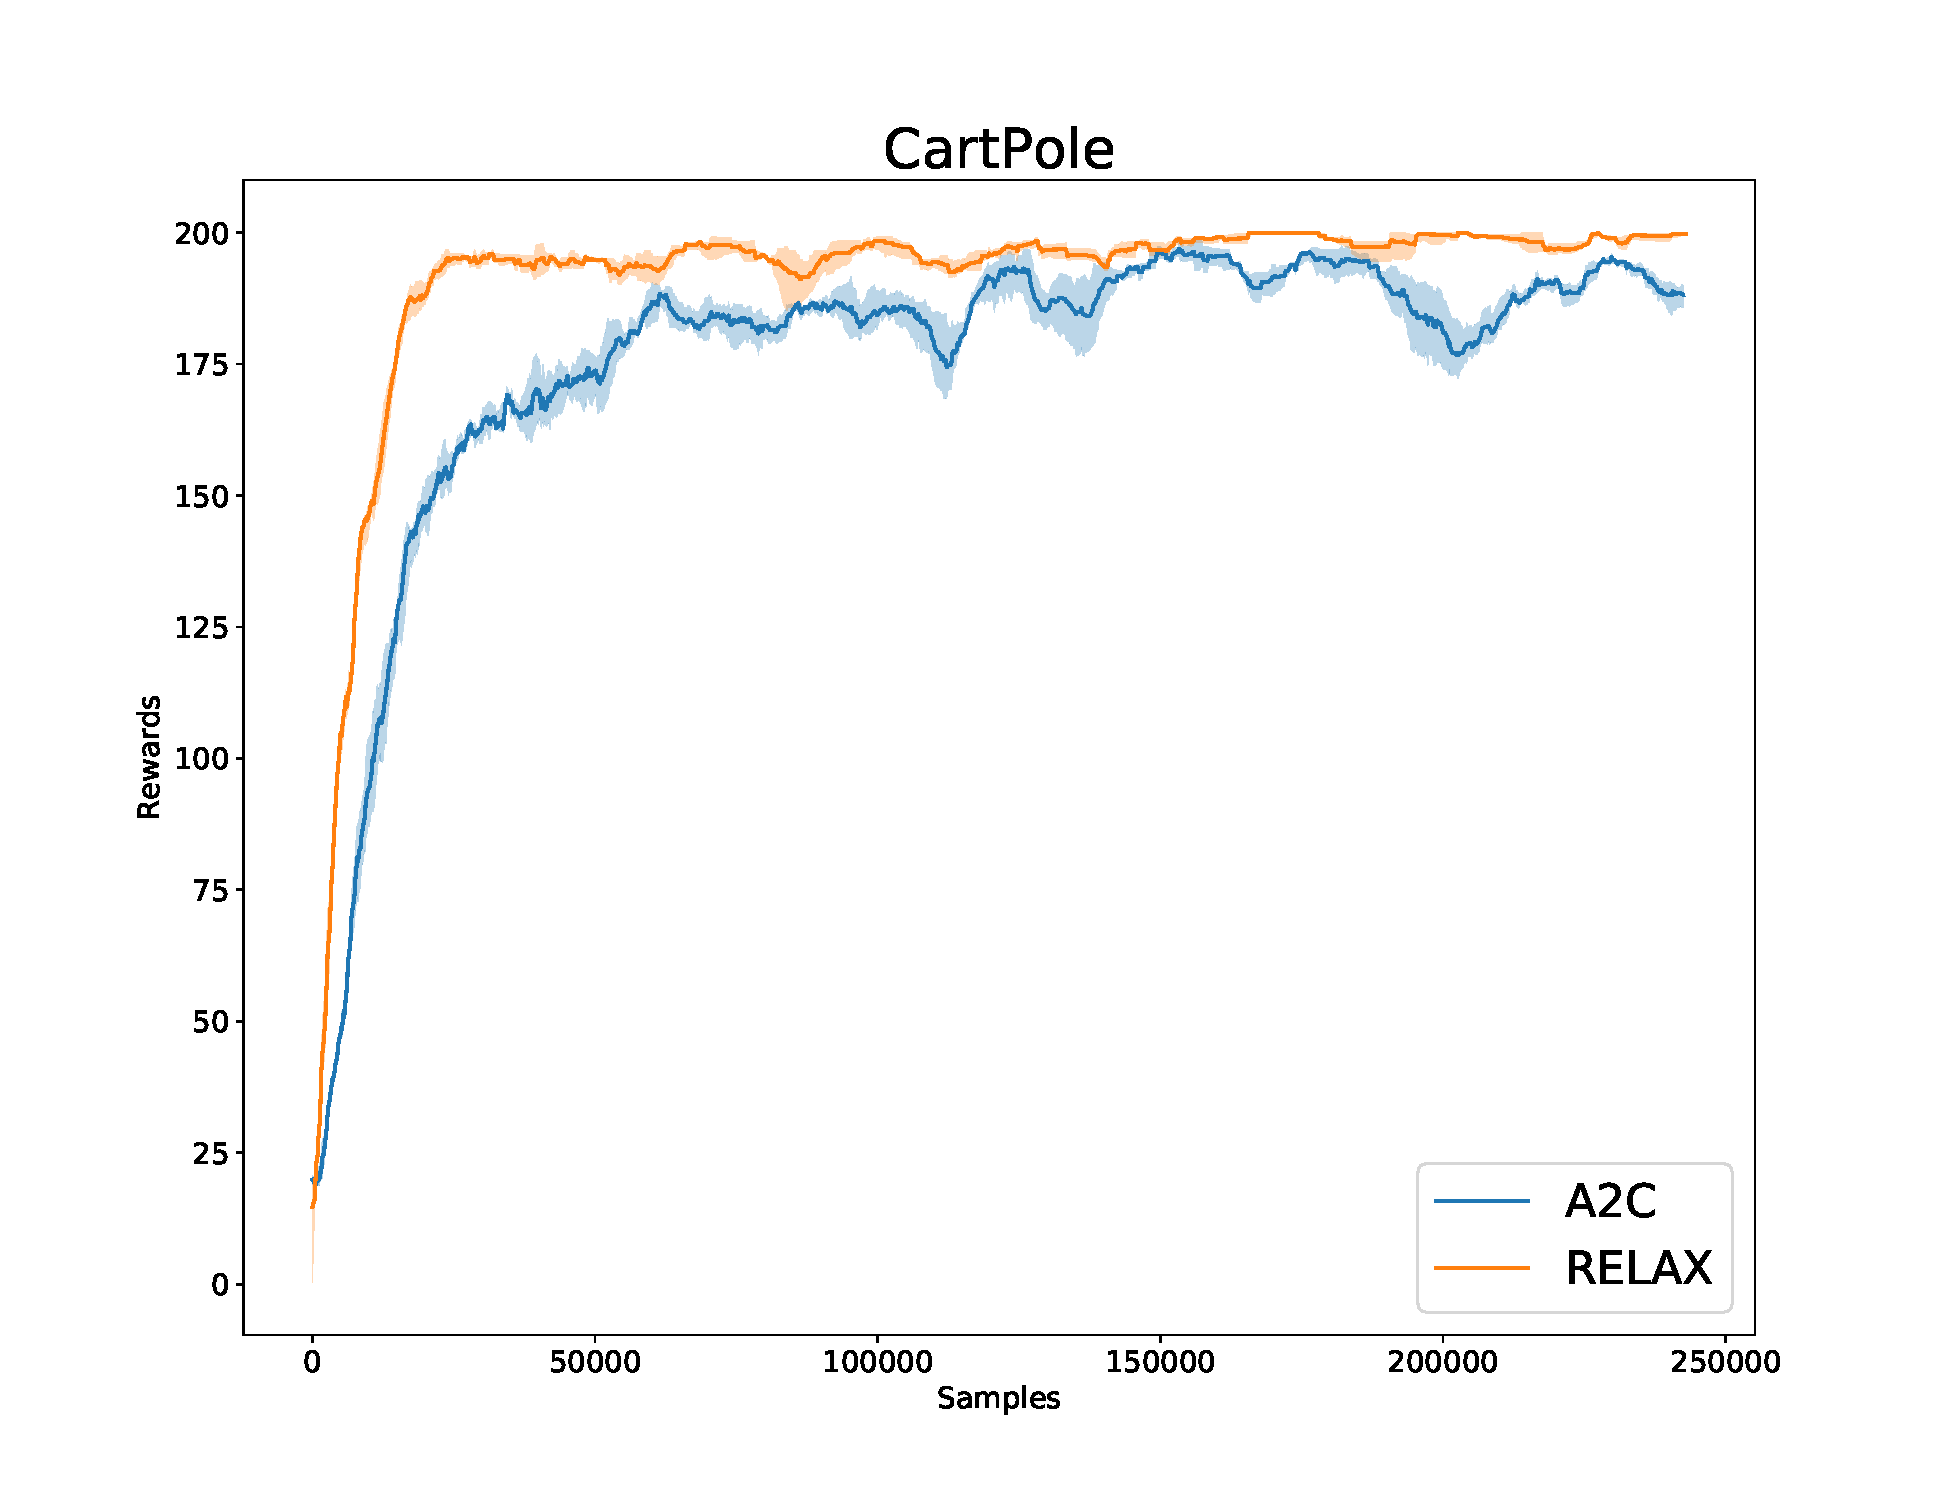
\includegraphics[width=.4\textwidth]{figures/cp_paper}
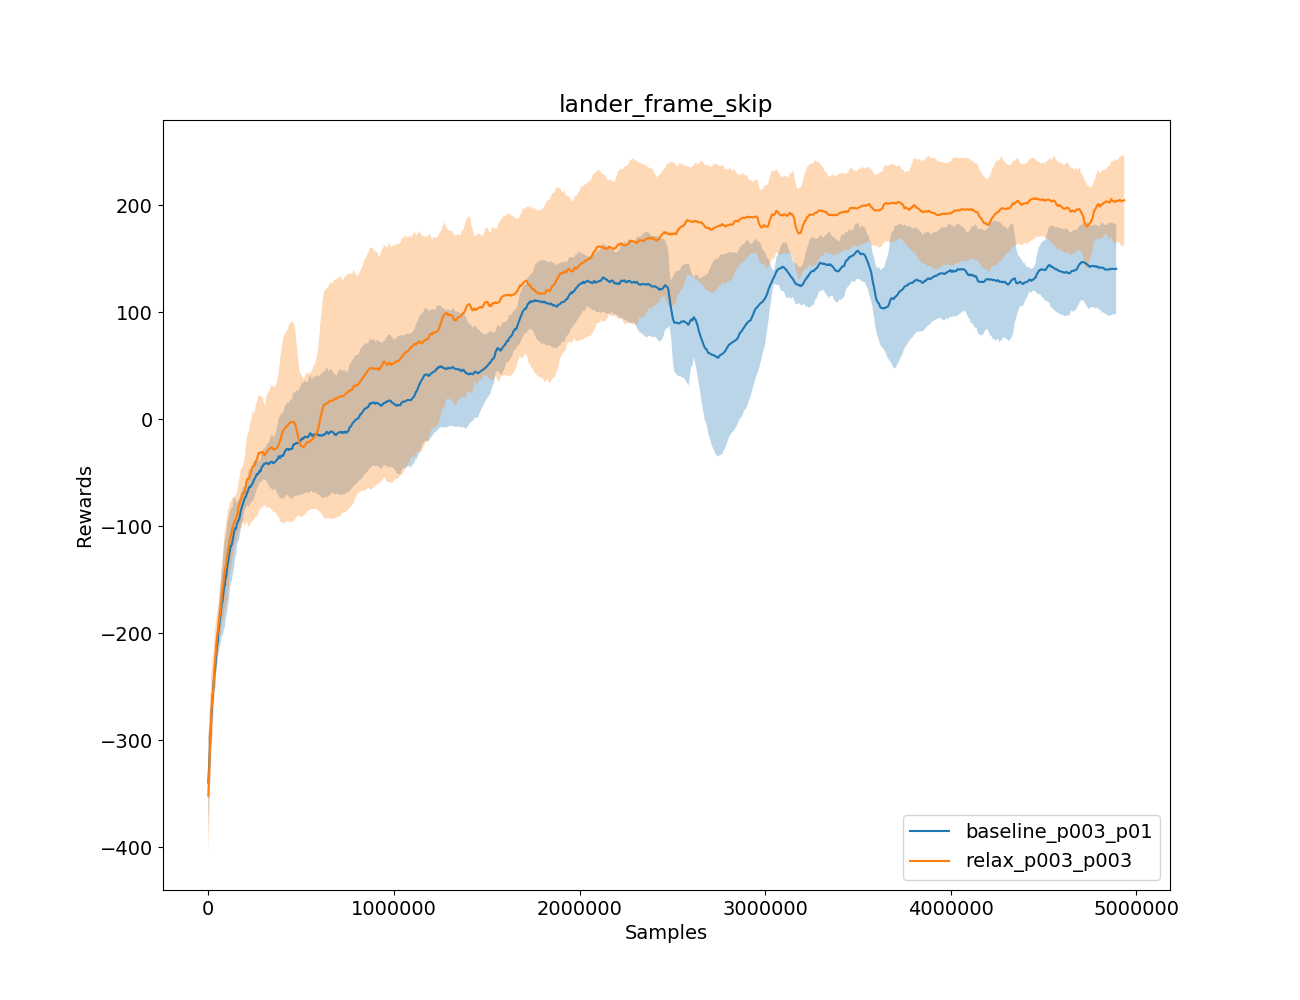
\includegraphics[width=.4\textwidth]{figures/lander_rewards}
\label{fig:disc_rl}
\end{center}
\caption{Discrete RL Experiments.}
\emph{Left:} CartPole.
\emph{Right:} LunarLander.

\end{figure}

\citet{mnih-dqn-2015}

[Do we use ADAM \citep{kingma2015adam} for optimization?]


\section{Conclusions and Future Work}
\label{conclusion}

In this work, synthesized and generalized many of the standard approaches for constructing gradient estimators.
We proposed a simple and generic gradient estimator that can be applied to expectations of known or black-box functions of discrete or continuous random variables. We also derive a simple extension to apply our method to reinforcement learning in both discrete and continuous action domains. 
This approach is relatively simple to implement and adds minimal computational overhead. 

The foundation of our approach is the score function gradient estimator with a control variate whose expectation can be estimated with low variance using the reparameterization trick.
This control variate is neural network which is trained directly to minimize the variance of the estimated gradients.
The central result of this paper is that learning the function in the control variate leads to even better convergence properties and lower variance gradient estimates. 


Other possible applications:

GANs \citep{goodfellow2014generative} that generate text or other discrete objects.

Learning to parse \citep{kusner2017grammar}

VAEs with continuous latent variables but non-differentiable likelihood functions.

%\section*{Acknowledgements}  % Uncomment for arxiv
%We thank Tian Qi Chen for helpful discussions.

\bibliography{bibliography}
\bibliographystyle{iclr2018_conference}



%\section{Appendix A: Control Variates}
% basic definitions following level of detail in Tucker 2017


% ** Questions to answer: 
% (1) is z-tilde a clever way of using Rao-Blackwellization for a part of the reparameterization gradient? This would mean that the reparameterization z-tilde is related to the sufficient statistic of the estimator...
% (1) also maybe: the Q function has the opportunity to learn an estimator based on the sufficient statistics of the model, which by Rao-Blackwell-Kolmogorov is lower variance
% (2) What's a better notation to keep the dependence of z on $\theta$ in view?
% (3) is the REBAR control variate really using the reparameterization gradient in a meaningful way? Or, is it best viewed as just another f + control variate where control variate is cleverly designed with lower variance? 


%\par{Generalizing the reparameterization trick}

%Write sample from distribution $s(\epsilon)$ as $\epsilon = \mathcal{T}^{-1}(\mathbf{z}; \mathbf{\nu})$ for some invertible transform $\mathcal{T}$ with variational parameters $\nu$.
%write out transformed density
%example: normal with standard normal $s$
%example: inverse CDF of Gaussian with uniform $s$
%write out expected gradient under transformation
%show decomposition of expected gradient into reparameterization and correction terms 

%\par{Applying GRG to REBAR}

%show mapping of terms
%note denser derivation in REBAR appendix

%\par{Interpreting REBAR through GRG}



\section{Appendix A: Conditional Re-sampling for Discrete Random Variables}
\label{resample}
When applying the RELAX estimator to a function of discrete random variables $b \sim p(b|\theta)$, we require that there exists a distribution $p(z|\theta)$ and a deterministic mapping $H(z)$ such that if $z \sim p(z|\theta)$ then $H(z) = b \sim p(b|\theta)$. Treating both $b$ and $z$ as random, this procedure defines a probabalistic model $p(b, z | \theta) = p(b|z)p(z|\theta)$. The RELAX estimator requires reparameterized samples from $p(z|\theta)$ and $p(z|b,\theta)$. We describe how to sample from these distributions in the common cases of $p(b|\theta) = \text{Bernoulli}(\theta)$ and $p(b|\theta) = \text{Categorical}(\theta)$.

\paragraph{Bernoulli} When $p(b|\theta)$ is Bernoulli distribution we let $H(z) = \mathbb{I}(z>0)$ and we sample from $p(z|\theta)$ with 
$$ z = \log \frac{\theta}{1 - \theta} + \log \frac{u}{1-u}, \qquad u \sim \text{uniform}[0,1].
$$ 
We can sample from $p(z|b, \theta)$ with 
\[
\tilde{z} =    \left\{
\begin{array}{ll}
      v\cdot\theta & b = 0 \\
      v(1-\theta) + \theta & b = 1 \\
\end{array} 
\right.
\]
where $v \sim \text{uniform}[0, 1]$.

\paragraph{Categorical} When $p(b|\theta)$ is a Categorical distribution where $\theta_i = p(b=i|\theta)$, we let $H(z) = \text{argmax}(z)$ and we sample from $p(z|\theta)$ with 
$$ z = \log\theta -\log(-\log u), \qquad u \sim \text{uniform}[0,1]^k
$$ where $k$ is the number of possible outcomes.

Intuitively, to sample from $p(z|b, \theta)$ we should first sample $v\sim \text{uniform}[0, 1]^k$, then compute $g_b = \log\theta_b -\log(-\log(v_b))$. Then we must determine how to scale each $v_{i\neq b}$ such that $g_{i\neq b} < g_b$. We can define $v'$ such that
\[
v_i' =    \left\{
\begin{array}{ll}
      v_i & i = b \\
      v_i\cdot(v_b)^{\frac{\theta_i}{\theta_b}} & i \neq b \\
\end{array} 
\right.
\] and then $\tilde{z} = \log\theta - \log(-\log v')$ which is our sample from $p(z|b, \theta)$. 

%Let $G_{1:k} = -\log-\log(U_{i:k})$ be samples from the Gumbel distribution, and learnable parameters $(\alpha_1, \dots, \alpha_k)$ be interpreted as some unnormalized parameterization of the discrete distribution under consideration.
%Then, consider the following sampling procedure: for each k, find the k that maximizes $\log \alpha_k - G_k$, and then set $D_k=1$ and $D_{i \neq k} = 0$. The Gumbel-Max trick states that sampling from the discrete distribution is equivalent to taking this argmax, that is, $p(D_k = 1) = \alpha_k / \sum_{i=1}^n \alpha_i$.

%Since taking an argmax is still a discontinuous operation, \cite{maddison2016concrete} and \cite{jang2016categorical} proposed further relaxing the argmax operator through the softmax function with an additional temperature parameter $\lambda$:
%\begin{equation}
%x_k = \frac{\exp\{( \log \alpha_k+ G_k) / \lambda\}}{\sum_{i=1}^n\exp\{( \log \alpha_i+ G_i) / \lambda\}}
%\end{equation}
%This relaxation allows values within the simplex, but in the low temperature limit, it becomes exactly the discrete argmax.
%One limitation of the concrete distribution is that it is a biased estimator except in limiting temperature.
%In other words, a small amount of bias is present for a non-zero temperature.

\section{Appendix B: RL proofs}

\paragraph{Proof 1}

We begin with 
\begin{align}
\E_\tau\Big[\frac{\partial m(a_t, s_t)}{\partial\theta}\Big] &= \E_{a_{1:t-1},s_{1:t}}\Big[E_{a_{t:T},s_{t+1:T}}\Big[\frac{\partial m(a_t, s_t)}{\partial\theta}\Big]\Big]\\
&= \E_{a_{1:t-1},s_{1:t}}\Big[E_{a_t}\Big[\frac{\partial m(a_t, s_t)}{\partial\theta}\Big]\Big]\\
&=  \E_{a_{1:t-1},s_{1:t}}\Big[\frac{\partial{E_{a_t}[m(a_t, s_t)]}}{\partial \theta}\Big]\\
&= \E_{a_{1:t-1},s_{1:t}}\Big[E_{a_t}\Big[\LL{t} m(a_t, s_t)\Big]\Big]\\
&= E_\tau\Big[\LL{t} m(a_t, s_t)\Big]
\end{align}
which completes our proof.

In the discrete action setting our policy parameterizes a soft-max distribution which we use to sample actions. 
In the discrete case we define $z_t = f(\pi, u) = \sigma (\log\pi - \log(-\log(u)))$ where $u\sim \text{Unif}[0, 1]$, $a_t = \text{argmax}(z_t)$, $\sigma$ is the soft-max function.

We also define $\tilde{z_t} \sim p(z_t|a_t)$ so if the $z_t$ are gumbel softmax samples, then $\tilde{z_t}$ are gumbel softmax samples constrainted so that the largest value is that of the index of $a_t$. See Appendix (section\ref{resample}) for how to efficiently generate samples $\tilde{z_t}$. 

In the discrete case, we use $m(\tilde{z_t}, s_t)\cdot \LL{t}$ as our control variate giving us $$\frac{\partial \E_\tau[R]}{\partial \theta} = \E_\tau\Big[\sum_{t=1}^T \LL{t} [(\sum_{t'=t}^T r_{t'}) - m(\tilde{z_t}, s_t)]\Big]$$ which is biased, so we must add a term to remove this bias which will be $\frac{\partial m(z_t, s_t)}{\partial\theta} - \frac{\partial m(\tilde{z_t}, s_t)}{\partial\theta}$ making the full estimator
$$\frac{\partial \E_\tau[R]}{\partial \theta} = \E_\tau\Big[\sum_{t=1}^T \LL{t} [(\sum_{t'=t}^T r_{t'}) - m(\tilde{z_t}, s_t)] + \frac{\partial m(z_t, s_t)}{\partial\theta} -  \frac{\partial m(\tilde{z_t}, s_t)}{\partial\theta}\Big].$$ 

For this estimator to be unbiased, we must have $$\E_\tau\Big[\sum_{t=1}^T \LL{t} m(\tilde{z_t}, s_t) - \Big(\frac{\partial m(z_t, s_t)}{\partial\theta} - \frac{\partial m(\tilde{z_t}, s_t)}{\partial\theta}\Big)\Big] = 0$$ and we claim that $\forall t$  $$\E_\tau\Big[ \LL{t} m(\tilde{z_t}, s_t) - \Big(\frac{\partial m(z_t, s_t)}{\partial\theta} - \frac{\partial m(\tilde{z_t}, s_t)}{\partial\theta}\Big)\Big] = 0$$ 

We introduce some notation that $a(z) = \text{argmax}(z)$

\begin{align}
0 = \PT \E_\tau\Big[ m(z_t, s_t) - m(z_t, s_t) \Big] = \E_{a_{<t},s_{\leq t}}\Big[ \PT \E_{z_t|s_t} \Big[ m(z_t, s_t) \Big] -  \PT \E_{a_t|s_t} \Big[ \E_{z_t|a_t, s_t}\Big[ m(z_t, s_t)\Big] \Big]\Big]
\end{align}
We drop the outer expectation for brevity and continue
\begin{align}
\PT \E_{z_t|s_t} &\Big[ m(z_t, s_t) \Big] -  \PT \E_{a_t|s_t} \Big[ \E_{z_t|a_t, s_t}\Big[ m(z_t, s_t)\Big] \Big]\\
&= \PT \E_{z_t|s_t} \Big[ m(z_t, s_t) \Big] - \E_{a_t|s_t} \Big[ \E_{z_t|a_t, s_t}\Big[m(z_t, s_t) \LL{t} -\PT \E_{z_t|a_t, s_t}\Big[m(z_t, s_t)  \Big] \Big]\\
&= \E_{z_t|s_t} \Big[ \PT m(z_t, s_t) \Big] - \E_{a_t|s_t} \Big[ \E_{z_t|a_t, s_t}\Big[m(z_t, s_t) \LL{t} - \E_{z_t|a_t, s_t}\Big[\PT m(z_t, s_t)  \Big] \Big]
\end{align}
Thus due to the markov property of the MDP, then we can wrap all of these expectations into the expectation over trajectories giving us

\begin{align}
\E_{a_{<t},s_{\leq t}}\Big[\E_{z_t|s_t} \Big[ \PT m(z_t, s_t) \Big] &- \E_{a_t|s_t} \Big[ \E_{z_t|a_t, s_t}\Big[m(z_t, s_t) \LL{t} - \E_{z_t|a_t, s_t}\Big[\PT m(z_t, s_t)  \Big] \Big]\Big]\\
&= \E_\tau\Big[ \LL{t} m(\tilde{z_t}, s_t) - \Big(\frac{\partial m(z_t, s_t)}{\partial\theta} - \frac{\partial m(\tilde{z_t}, s_t)}{\partial\theta}\Big)\Big] = 0
\end{align}

%We can estimate this value with the REINFORCE gradient estimator as $$\frac{\partial \mathbb{E}_{\pi(a|\phi)}[f(a)]}{\partial \phi} = \mathbb{E}[f(a)\frac{\partial \log p(a)}{\partial \phi}]$$ but the variance of this estimator can be very high thus making our model very sample-inefficient. We can subtract a control variate $r(\rho)\frac{\partial \log p(a(\rho))}{\partial \phi}$ where $\rho$ is sampled from some distribution which is a function of $\phi$ and $a(\rho)$ is a deterministic function of such that $a \sim \pi(a|\phi)$.

\section{Appendix C: Experimental Details}
\subsection{Discrete VAE}
We run all models for $2,000,000$ iterations with a batch size of $24$. For the REBAR models, we tested learning rates in $\{.005, .001, .0005,  .0001, .00005\}$. 

RELAX adds more hyperparameters. These are the depth of the neural network component of our control variate $r_\rho$, the weight decay placed on the network, and the scaling on the learning rate for the control variate. We tested neural network models with $l$ layers of 200 units using the ReLU nonlinearity with $l \in \{2, 4\}$. We trained the control variate with weight decay in $\{.001, .0001\}$. We trained the control variate with learning rate scaling in $\{1, 10\}$.

To limit the hyperparameter search and to demonstrate the impact of reduced-variance gradient estimates, we choose the base learning rate for RELAX to be the best performing learning rate from REBAR. We believe further improvement could be achieved by tuning this parameter.

All presented results are from the models which achieve the highest ELBO on the validation data.


\subsubsection{Two layer model}
In the two layer models we optimize the ELBO $$\mathcal{L}(\theta) = \E_{q(b_2|b_1)q(b_1|x)}[\log p(x|b_1) + \log p(b_1|b_2) + \log p(b_2) - \log q(b_1|x) - \log q(b_2|b_1)]$$ where $q(b_1|x) = \sigma(x\cdot W_{q_1} + \beta_{q_1})$, $q(b_2|b_1) = \sigma(b_1\cdot W_{q_2} + \beta_{q_2})$, $p(x| b_1) = \sigma(b_1\cdot W_{p_1} + \beta_{p_1})$, and $p(b_1| b_2) = \sigma(b_2\cdot W_{p_2} + \beta_{p_2})$ with weight matrices $W$ and biases $\beta$. As in the one layer model, the prior $p(b_2)$ is also learned.



\label{app_disc_vae}
\subsection{Discrete RL}
\subsection{Continuous RL}

\end{document}
